\documentclass[14pt]{extreport}
\usepackage{gost}
\usepackage{hyperref}
\usepackage{makecell}
\usepackage{ragged2e}
\usepackage{graphicx}%Вставка картинок правильная
\usepackage{float}%"Плавающие" картинки
\usepackage{wrapfig}%Обтекание фигур (таблиц, картинок и прочего)
\justifying
\makeatletter
\@addtoreset{figure}{part}% Reset figure numbering at every part
\makeatother
\renewcommand{\thefigure}{\arabic{figure}}% Figure number is part.figure
\renewcommand{\thetable}{\arabic{table}}



%Тут можно вставить дополнительные пакеты

\begin{document}
\pagestyle{empty} %  выключаем нумерацию

\includepdf[pages=-,pagecommand={}]{title_page.pdf}


\pagestyle{plain} % включаем нумерацию
\tableofcontents
\intro\label{intro}

Данный отчет содержит в себе основную идею будующей информационной системы с рабочим названием MEET ME, планируемый набор ее функций, основных пользователей этой информациионной системы, прототип интерфейса, а так же анализ рынка.

\chapter{ОПИСАНИЕ ИДЕИ ИНФОРМАЦИОННОЙ СИСТЕМЫ \label{chapter1}}

\section{Основной функционал }

Информационная система MEET ME представляет из себя веб-приложение для планирования встреч с друзьями и родственниками в виде календаря. 
Приложение показывает пересечение свободного времени пользователя с одним или несколькими его друзьями.
C помощью данного приложения пользователь может эффективно планировать встречи со своими друзьями, родственниками или знакомыми не тратя огромное количество времени на согласования времени. 

После создания аккаунта, пользователю будет предложено настроить свое расписание. Пользователь выбирает дни и время, когда он имеет возможность для встречи. Планируется реализация возможности определения свободных промежутков с помощью импорта данных с Google Calendar и аналогов, а так же .cal файлов.
Пользователь может настроить свое расписание как на неделю, так и на месяц вперед. Настроив свое расписание, пользователь должен добавить своих друзей.  Добавление друзей идет посредством отправки запроса другу на его электронную почту указаную при регистрации аккаунта. Добавив своих друзей, пользователь может создать группу из друзей, если они планируют встречаться вместе.

Настроив свое расписание и добавив друзей, пользователю начинают отображаться пересечения в расписании с его друзьями в виде календаря. Пользователю не показывается полностью расписание встреч его друзей ради сохранения приватности. Пользователь может отправить приглашение на встречу своему другу если их свободное время пересекается в приложении. Приглашение отобразится у его друга и он сможет принять или отклонить его. Приняв приглашение у обоих пользователей отобразится встреча в их календаре. Так же пользователь может создать группу из друзей. Создав группу, она будет отображаться в пересечениях вместе с друзьями. Рядом с названием группы будет отображаться количество друзей из группы, для которых это врем свободно. Участники группы могут утвердить время встречи методом голосования и тогда встреча будет отображаться в расписании остальных участников группы, они смогут присоединиться к мероприятию нажав на соответствующую кнопку.

Подводя итоги, приложение будет иметь следующий функционал 
\begin{itemize}
    \item Регистрация аккаунта;
    \item Настройка свободного времени вручную;
    \item Настройка свободного времени основываясь на рекомендациях данных системой благодаря импорту расписания из Google Calendar / .cal файлов;
    \item Редактирование свободного времени;
    \item Отправка и принятие заявок в друзья;
    \item Создание группы из существующих друзей;
    \item Отправка приглашений на встречу;
    \item Принятие/Отклонение встречи;
    \item Утверждение групповой встречи методом голосования.
\end{itemize}
\section{Основные пользователи  }

Информационная система будет иметь только прямых конечных пользователей. Система не требует модераторов, менеджеров и прочих пользователей.
Целевая аудитория данной информационной системы достаточно широка. Основными пользователями будут молодые, общительные люди, которые стараются грамотно распределять свое время (ученики старших классов, студенты, работающая молодежь).

\newpage
\section{Прототип интерфейса}
В данном разделе демонстрируется прототип веб-приложения для компьютеров (Рисунок \ref{fig:prototype}). Интерфейс состоит из боковой панели, календаря и элементов управления. На боковой панели присутствует название приложения, кнопка <<изменить>>, которая позволяет изменять собственное расписание, список друзей, кнопка позваляющая добавить нового друга. Ниже располагается список компаний, а так же кнопка позоляющая создать новую. При наличии активных приглашений, они будут отображаться снизу. Их можно будет принять или отклонить нажав на соответствующую кнопку.
Сверху находятся элементы управления. Пользователь может выбрать отображение календаря на неделю, месяц или 3 дня. Используя соответствующие кнопки пользователь может перемещаться на выбранный период. Так же сверху находятся настройки аккаунта, в которые пользователь может попасть кликнув на свое имя.
\begin{figure}[h]   
    \centering
    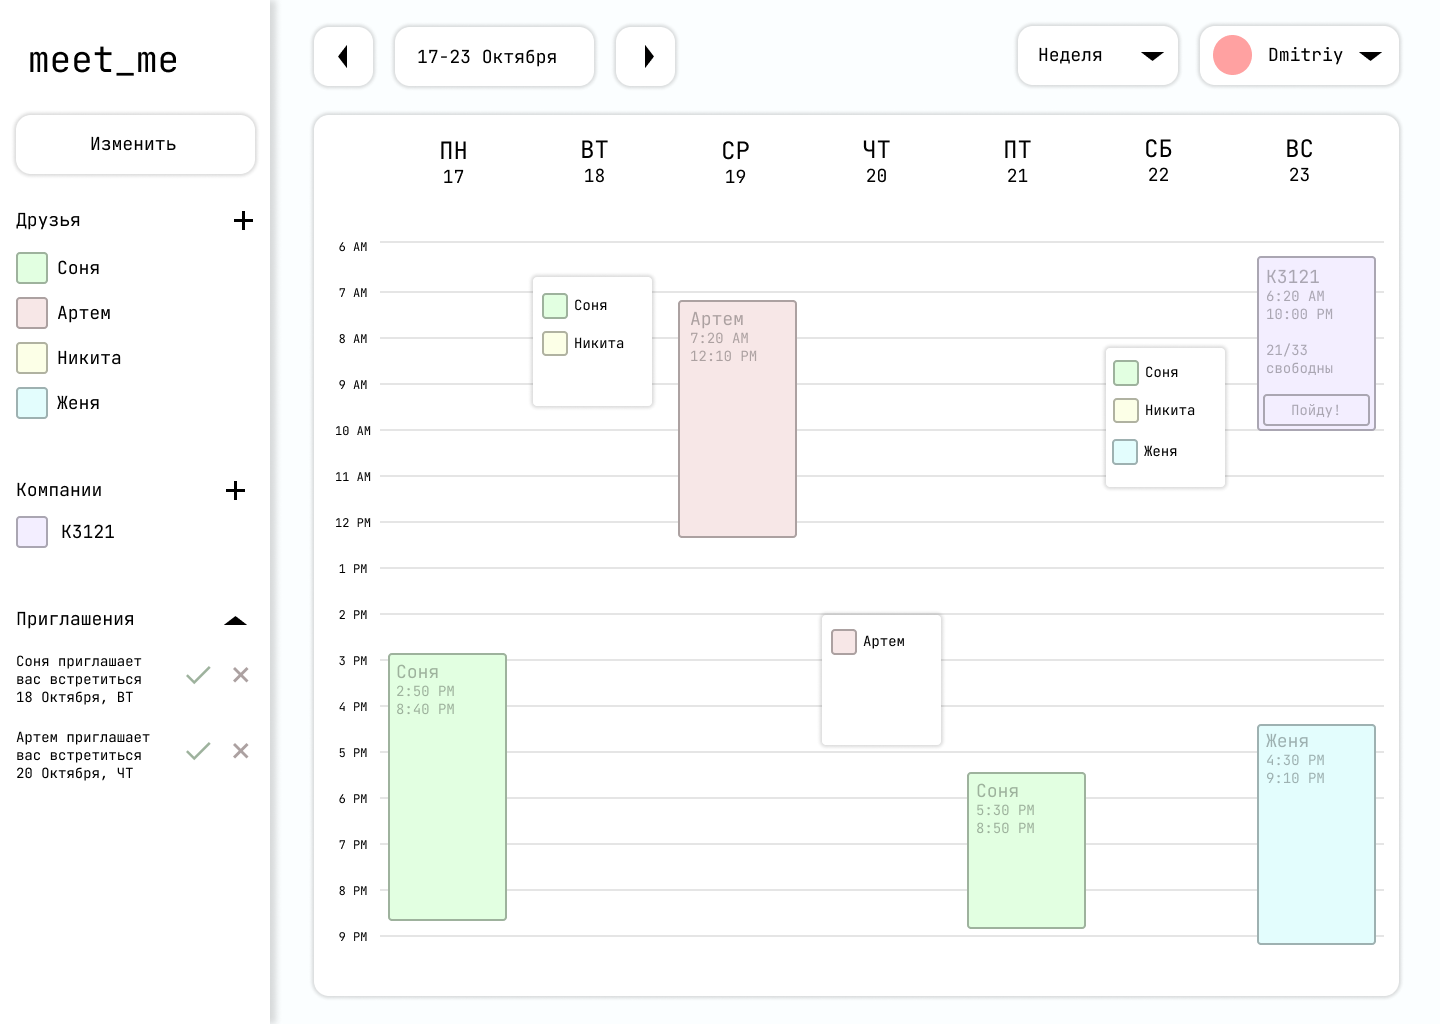
\includegraphics[width=0.9\linewidth]{prototype.png}
    \caption{ Прототип интерфейса}
    \label{fig:prototype}
\end{figure}

Основная часть интерфейса выполнена в виде календаря. Календарь размечен по дням и времени.
На календаре, тем же цветом, что и в боковой панели, отображаются уже согласованные встречи с друзьями. Белым же цветом отображаются пересечения свободного времени с друзьями. В блоке пересечений отображаются друзья, с которыми свободное время пересекается.
Нажав на имя друга, пользователю будет предложено отправить приглашение другу на это свободное время.

\chapter{АНАЛИЗ РЫНКА \label{chapter2}}
\section{Обзор аналогов, представленных на рынке}
Проведя анализ российского и зарубежного рынка, аналогов обнаружено не было. Существует несколько систем имеющих частично похожий функционал. 
В отличии от представленных ниже систем, система представленная в данном отчете ориентируется на использование людьми для ведения их личной жизни, а не для рабочих нужд. Так же система не завязана на одном пользователе создавшем опрос и может равноправно использоваться всеми участниками.
\subsection{NeedToMeet}
Сервис NeetToMeet \eqref{a:NeetToMeet} предоставляет возможность пользователям создавать опросы, благодаря которым можно выбрать время и место для встречи. Сервис предоставляет ограниченное количество возможностей в бесплатной версии, полная версия стоит 20\$/год. Сервис в основном ориентируется на корпоративный сегмент. 
\subsection{Rally}
Сервис Rally \eqref{b:Rally} имеет схожих функционал с сервисом NeedToMeet, но в отличии от него бесплатен, имеет открытый исходный код, а так же для его использования не нужно регистрировать аккаунт. Пользователь так же создает опрос, а другие пользователи выбирают удобное время для встречи. 
\subsection{WhenAvalible}
Используя сервис WhenAvalible \eqref{c:WhenAvalible} пользователь создает опрос, а другие пользователи подтверждают свою возможность встретиться в тот или иной день. Сервис предоставляет ограниченный функционал в бесплатной версии, платная версия стоит 38\$/год.

\section{Обоснование необходимости разработки информационной системы }
Проведя анализ рынка, можно сделать вывод, что идея уникальна. Аналогов на рынке не найдено, а те сервисы, что имеют частично схожий функционал - завязаны вокруг одного пользователя, который создает опрос. 


\chapter{ЗАКЛЮЧЕНИЕ \label{chapter3}}
Был составлен отчет, сформулирована основная идея будущей информационной системы. Описан основной функционал системы, основные пользователи, создан прототип интерфейса, а так же был проведен анализ рынка и приведено описание аналогов.
\chapter{СПИСОК ИСПОЛЬЗОВАННЫХ ИСТОЧНИКОВ \label{chapter4}}
\begin{enumerate}
    \item \label{a:NeetToMeet} NeedToMeet: официальный сайт. URL: \url{https://www.needtomeet.com} (Дата обращения 19.10.2022)
    \item \label{b:Rally} Rally: официальный сайт. URL: \url{https://rallly.co/} (Дата обращения 19.10.2022)
    \item \label{c:WhenAvalible} WhenAvalible: официальный сайт. URL: \url{https://whenavailable.com/} (Дата обращения 19.10.2022)
\end{enumerate}
% \newpage
\end{document}
